L'objectif dans cette partie est de créer une interface interactive entre le joueur et le système. Nous voulons que le joueur puisse avancer ou reculer au sens de l’évaluation entre les states comme il le souhaite.

\subsubsection{Couche principale}

Le fichier \textit{main.ts} est une interface entre notre évaluateur et la couche graphique. Nous implémentons les fonctions qui permettent cette navigation entre les state.

Pour cela nous implémentons la seule variable mutable du programme : \texttt{stateStack}. Il s’agit d’une pile de \textit{State} qui maintient l’historique de states. Il est important ici qu'elle soit mutable car les fonctions à suivre modifient l'historique à chaque interaction, et cette pile doit être dans une addresse global constante pour être référencé par les fonctions à suivre. 

\`A l’état initiale, \texttt{stateStack} est la pile contenant seulement le initial state et, à tout moment, head de \texttt{stateStack} est le state courant : les states s’empile gardant le plus récent au-dessus.

Trois fonction manipulent \texttt{stateStack}:
\begin{itemize} 
\item \texttt{step} : avance d'un pas en appliquant \texttt{popStateStack} au head de \texttt{stateStack} et empile le nouvel état sur \texttt{stateStack}, on doit vérifier d’abord que on est pas dans un state finale pour l'utliser; 
\item \texttt{back} : recule d'un pas en dépilant \texttt{stateStack} et renvoyant head, attention car si \texttt{stateStack} est vide alors on peut plus rien faire ainsi, par sécurité, si nous somme dans l’état initiale nous renvoyons head sans dépiler; 
\item \texttt{restart} : reinitialise \texttt{stateStack} à l'état initial. 
\end{itemize}

La fonction \texttt{stateToUI} assure la conversion d'un \textit{State} en \textit{StateUI}, une représentation simplifiée destinée à l'afficheur. Cette couche de séparation garantit que la logique du jeu reste indépendante de toute décision d'affichage..

\subsubsection{Afficheur}

L'afficheur reçoit des \textit{StateUI} et met à jour le DOM en conséquence. Le plateau est rendu sous forme de tableau HTML, chaque case portant une classe CSS selon sa couleur. Le robot est représenté par une police d'icônes personnalisée (\texttt{robots.ttf}), définissant seize glyphes dont quatre orientations du robot et une étoile.

Quatre boutons permettent l'interaction : 
\begin{itemize}
  \item \textit{step} pour avancer : on appelle \texttt{step} en verifiant \texttt{!isEnd}, recevons un \textit{StateUI} puis actualisons le DOM;
  \item \textit{back} pour reculer : on appelle \texttt{back} et actualisons;
  \item \textit{play} pour exécuter automatiquement pas à pas avec un délai de 100ms jusqu’à arriver dans un state finale;
  \item \textit{restart} pour réinitialiser. L'afficheur délègue entièrement la logique à \texttt{main.ts} et ne manipule que la présentation.
\end{itemize}

\begin{figure}[H]
    \centering
    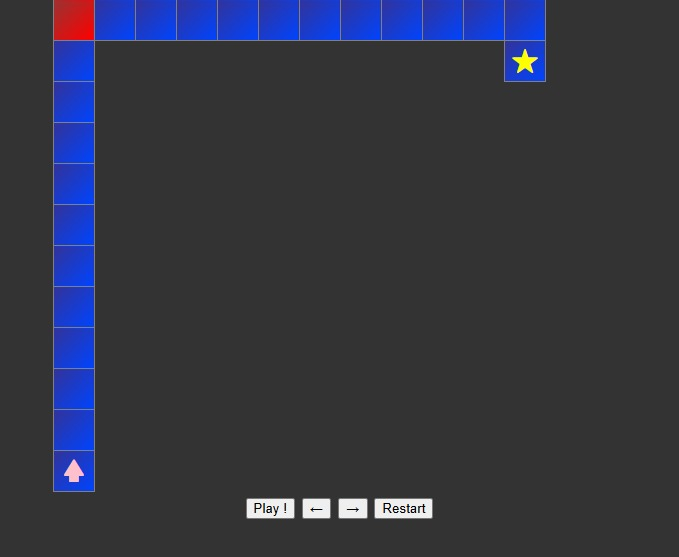
\includegraphics[width=0.6\textwidth]{interface.jpeg}
    \caption{Interface graphique projet robozzle}
    \label{fig:ui}
\end{figure}

